% Created by tikzDevice version 0.12.6 on 2026-07-03 11:54:56
% !TEX encoding = UTF-8 Unicode
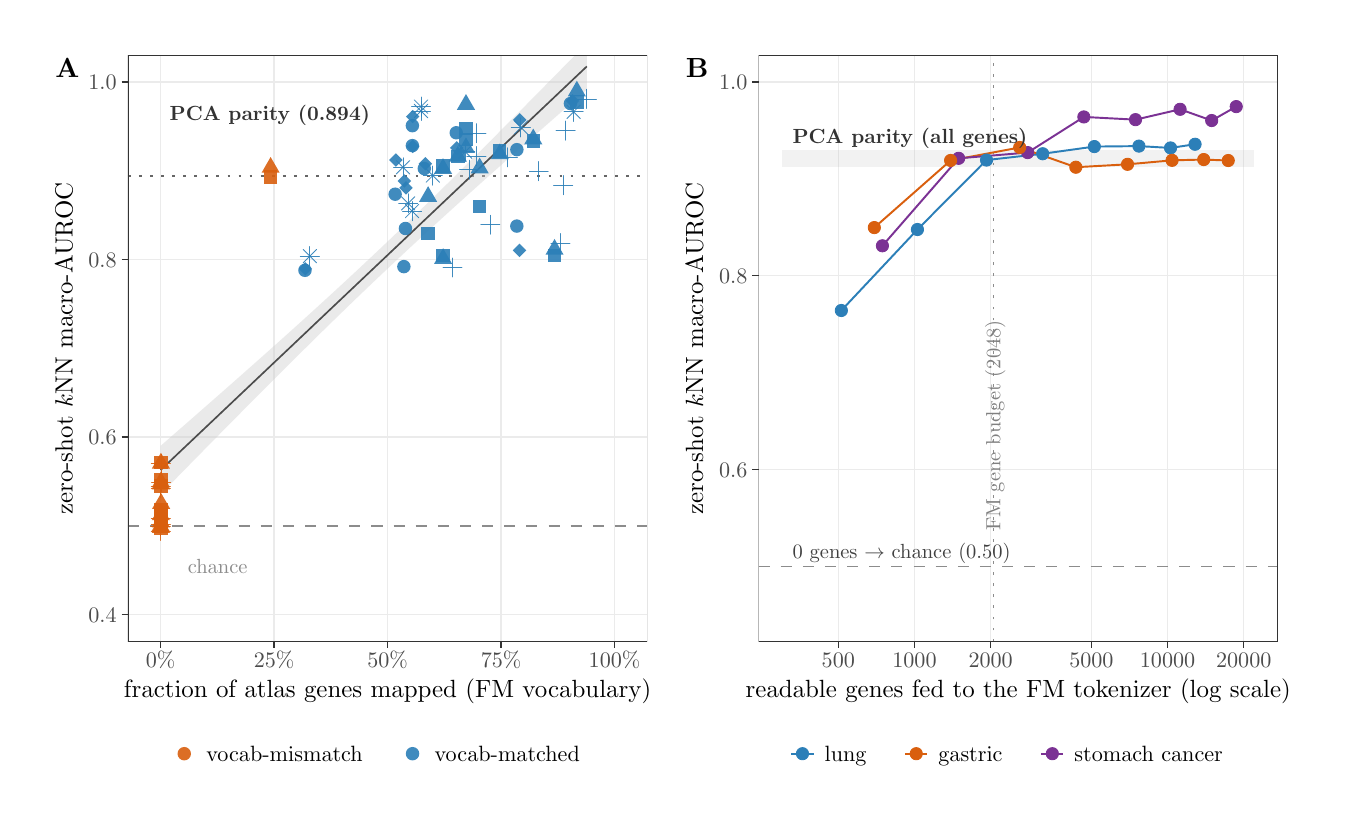
\begin{tikzpicture}[x=1pt,y=1pt]
\definecolor{fillColor}{RGB}{255,255,255}
\path[use as bounding box,fill=fillColor,fill opacity=0.00] (0,0) rectangle (469.75,281.85);
\begin{scope}
\path[clip] (  0.00,  0.00) rectangle (469.75,281.85);
\definecolor{drawColor}{RGB}{255,255,255}
\definecolor{fillColor}{RGB}{255,255,255}

\path[draw=drawColor,line width= 0.5pt,line join=round,line cap=round,fill=fillColor] (  0.00, -0.00) rectangle (469.75,281.85);
\end{scope}
\begin{scope}
\path[clip] (  5.00,  5.00) rectangle (232.88,276.85);
\definecolor{drawColor}{RGB}{255,255,255}
\definecolor{fillColor}{RGB}{255,255,255}

\path[draw=drawColor,line width= 0.5pt,line join=round,line cap=round,fill=fillColor] (  5.00,  5.00) rectangle (232.88,276.85);
\end{scope}
\begin{scope}
\path[clip] (232.88,  5.00) rectangle (460.75,276.85);
\definecolor{drawColor}{RGB}{255,255,255}
\definecolor{fillColor}{RGB}{255,255,255}

\path[draw=drawColor,line width= 0.5pt,line join=round,line cap=round,fill=fillColor] (232.88,  5.00) rectangle (460.76,276.85);
\end{scope}
\begin{scope}
\path[clip] ( 36.22, 60.07) rectangle (223.88,271.85);
\definecolor{fillColor}{RGB}{255,255,255}

\path[fill=fillColor] ( 36.22, 60.07) rectangle (223.88,271.85);
\definecolor{drawColor}{gray}{0.92}

\path[draw=drawColor,line width= 0.5pt,line join=round] ( 36.22, 69.69) --
	(223.88, 69.69);

\path[draw=drawColor,line width= 0.5pt,line join=round] ( 36.22,133.87) --
	(223.88,133.87);

\path[draw=drawColor,line width= 0.5pt,line join=round] ( 36.22,198.05) --
	(223.88,198.05);

\path[draw=drawColor,line width= 0.5pt,line join=round] ( 36.22,262.23) --
	(223.88,262.23);

\path[draw=drawColor,line width= 0.5pt,line join=round] ( 48.03, 60.07) --
	( 48.03,271.85);

\path[draw=drawColor,line width= 0.5pt,line join=round] ( 89.04, 60.07) --
	( 89.04,271.85);

\path[draw=drawColor,line width= 0.5pt,line join=round] (130.05, 60.07) --
	(130.05,271.85);

\path[draw=drawColor,line width= 0.5pt,line join=round] (171.06, 60.07) --
	(171.06,271.85);

\path[draw=drawColor,line width= 0.5pt,line join=round] (212.07, 60.07) --
	(212.07,271.85);
\definecolor{drawColor}{gray}{0.55}

\path[draw=drawColor,line width= 0.5pt,dash pattern=on 4pt off 4pt ,line join=round] ( 36.22,101.78) -- (223.88,101.78);
\definecolor{drawColor}{gray}{0.40}

\path[draw=drawColor,line width= 0.5pt,dash pattern=on 1pt off 3pt ,line join=round] ( 36.22,228.21) -- (223.88,228.21);
\definecolor{fillColor}{RGB}{204,204,204}

\path[fill=fillColor,fill opacity=0.40] ( 48.03,130.73) --
	( 49.98,132.43) --
	( 51.93,134.13) --
	( 53.88,135.84) --
	( 55.83,137.54) --
	( 57.78,139.24) --
	( 59.73,140.95) --
	( 61.68,142.66) --
	( 63.63,144.37) --
	( 65.58,146.08) --
	( 67.53,147.79) --
	( 69.48,149.50) --
	( 71.43,151.22) --
	( 73.38,152.94) --
	( 75.33,154.66) --
	( 77.28,156.38) --
	( 79.23,158.11) --
	( 81.18,159.84) --
	( 83.13,161.57) --
	( 85.08,163.30) --
	( 87.03,165.04) --
	( 88.98,166.78) --
	( 90.93,168.52) --
	( 92.88,170.27) --
	( 94.83,172.02) --
	( 96.78,173.78) --
	( 98.73,175.54) --
	(100.68,177.31) --
	(102.62,179.07) --
	(104.57,180.85) --
	(106.52,182.63) --
	(108.47,184.41) --
	(110.42,186.20) --
	(112.37,188.00) --
	(114.32,189.80) --
	(116.27,191.61) --
	(118.22,193.42) --
	(120.17,195.24) --
	(122.12,197.07) --
	(124.07,198.90) --
	(126.02,200.74) --
	(127.97,202.58) --
	(129.92,204.43) --
	(131.87,206.29) --
	(133.82,208.16) --
	(135.77,210.03) --
	(137.72,211.91) --
	(139.67,213.79) --
	(141.62,215.68) --
	(143.57,217.57) --
	(145.52,219.48) --
	(147.47,221.38) --
	(149.42,223.29) --
	(151.37,225.21) --
	(153.32,227.13) --
	(155.27,229.06) --
	(157.22,230.99) --
	(159.17,232.93) --
	(161.12,234.87) --
	(163.07,236.81) --
	(165.02,238.76) --
	(166.97,240.71) --
	(168.92,242.66) --
	(170.87,244.62) --
	(172.82,246.58) --
	(174.76,248.54) --
	(176.71,250.51) --
	(178.66,252.48) --
	(180.61,254.45) --
	(182.56,256.42) --
	(184.51,258.40) --
	(186.46,260.38) --
	(188.41,262.36) --
	(190.36,264.34) --
	(192.31,266.32) --
	(194.26,268.31) --
	(196.21,270.29) --
	(198.16,272.28) --
	(200.11,274.27) --
	(202.06,276.26) --
	(202.06,259.46) --
	(200.11,257.76) --
	(198.16,256.05) --
	(196.21,254.35) --
	(194.26,252.64) --
	(192.31,250.93) --
	(190.36,249.22) --
	(188.41,247.51) --
	(186.46,245.80) --
	(184.51,244.08) --
	(182.56,242.37) --
	(180.61,240.65) --
	(178.66,238.93) --
	(176.71,237.20) --
	(174.76,235.47) --
	(172.82,233.75) --
	(170.87,232.01) --
	(168.92,230.28) --
	(166.97,228.54) --
	(165.02,226.80) --
	(163.07,225.05) --
	(161.12,223.30) --
	(159.17,221.55) --
	(157.22,219.79) --
	(155.27,218.03) --
	(153.32,216.26) --
	(151.37,214.49) --
	(149.42,212.72) --
	(147.47,210.94) --
	(145.52,209.15) --
	(143.57,207.36) --
	(141.62,205.56) --
	(139.67,203.76) --
	(137.72,201.95) --
	(135.77,200.13) --
	(133.82,198.31) --
	(131.87,196.48) --
	(129.92,194.65) --
	(127.97,192.81) --
	(126.02,190.96) --
	(124.07,189.11) --
	(122.12,187.25) --
	(120.17,185.38) --
	(118.22,183.51) --
	(116.27,181.63) --
	(114.32,179.74) --
	(112.37,177.85) --
	(110.42,175.95) --
	(108.47,174.05) --
	(106.52,172.14) --
	(104.57,170.23) --
	(102.62,168.31) --
	(100.68,166.38) --
	( 98.73,164.46) --
	( 96.78,162.52) --
	( 94.83,160.59) --
	( 92.88,158.64) --
	( 90.93,156.70) --
	( 88.98,154.75) --
	( 87.03,152.80) --
	( 85.08,150.84) --
	( 83.13,148.88) --
	( 81.18,146.92) --
	( 79.23,144.96) --
	( 77.28,142.99) --
	( 75.33,141.02) --
	( 73.38,139.05) --
	( 71.43,137.08) --
	( 69.48,135.10) --
	( 67.53,133.12) --
	( 65.58,131.14) --
	( 63.63,129.16) --
	( 61.68,127.17) --
	( 59.73,125.19) --
	( 57.78,123.20) --
	( 55.83,121.21) --
	( 53.88,119.22) --
	( 51.93,117.23) --
	( 49.98,115.24) --
	( 48.03,113.25) --
	cycle;

\path[] ( 48.03,130.73) --
	( 49.98,132.43) --
	( 51.93,134.13) --
	( 53.88,135.84) --
	( 55.83,137.54) --
	( 57.78,139.24) --
	( 59.73,140.95) --
	( 61.68,142.66) --
	( 63.63,144.37) --
	( 65.58,146.08) --
	( 67.53,147.79) --
	( 69.48,149.50) --
	( 71.43,151.22) --
	( 73.38,152.94) --
	( 75.33,154.66) --
	( 77.28,156.38) --
	( 79.23,158.11) --
	( 81.18,159.84) --
	( 83.13,161.57) --
	( 85.08,163.30) --
	( 87.03,165.04) --
	( 88.98,166.78) --
	( 90.93,168.52) --
	( 92.88,170.27) --
	( 94.83,172.02) --
	( 96.78,173.78) --
	( 98.73,175.54) --
	(100.68,177.31) --
	(102.62,179.07) --
	(104.57,180.85) --
	(106.52,182.63) --
	(108.47,184.41) --
	(110.42,186.20) --
	(112.37,188.00) --
	(114.32,189.80) --
	(116.27,191.61) --
	(118.22,193.42) --
	(120.17,195.24) --
	(122.12,197.07) --
	(124.07,198.90) --
	(126.02,200.74) --
	(127.97,202.58) --
	(129.92,204.43) --
	(131.87,206.29) --
	(133.82,208.16) --
	(135.77,210.03) --
	(137.72,211.91) --
	(139.67,213.79) --
	(141.62,215.68) --
	(143.57,217.57) --
	(145.52,219.48) --
	(147.47,221.38) --
	(149.42,223.29) --
	(151.37,225.21) --
	(153.32,227.13) --
	(155.27,229.06) --
	(157.22,230.99) --
	(159.17,232.93) --
	(161.12,234.87) --
	(163.07,236.81) --
	(165.02,238.76) --
	(166.97,240.71) --
	(168.92,242.66) --
	(170.87,244.62) --
	(172.82,246.58) --
	(174.76,248.54) --
	(176.71,250.51) --
	(178.66,252.48) --
	(180.61,254.45) --
	(182.56,256.42) --
	(184.51,258.40) --
	(186.46,260.38) --
	(188.41,262.36) --
	(190.36,264.34) --
	(192.31,266.32) --
	(194.26,268.31) --
	(196.21,270.29) --
	(198.16,272.28) --
	(200.11,274.27) --
	(202.06,276.26);

\path[] (202.06,259.46) --
	(200.11,257.76) --
	(198.16,256.05) --
	(196.21,254.35) --
	(194.26,252.64) --
	(192.31,250.93) --
	(190.36,249.22) --
	(188.41,247.51) --
	(186.46,245.80) --
	(184.51,244.08) --
	(182.56,242.37) --
	(180.61,240.65) --
	(178.66,238.93) --
	(176.71,237.20) --
	(174.76,235.47) --
	(172.82,233.75) --
	(170.87,232.01) --
	(168.92,230.28) --
	(166.97,228.54) --
	(165.02,226.80) --
	(163.07,225.05) --
	(161.12,223.30) --
	(159.17,221.55) --
	(157.22,219.79) --
	(155.27,218.03) --
	(153.32,216.26) --
	(151.37,214.49) --
	(149.42,212.72) --
	(147.47,210.94) --
	(145.52,209.15) --
	(143.57,207.36) --
	(141.62,205.56) --
	(139.67,203.76) --
	(137.72,201.95) --
	(135.77,200.13) --
	(133.82,198.31) --
	(131.87,196.48) --
	(129.92,194.65) --
	(127.97,192.81) --
	(126.02,190.96) --
	(124.07,189.11) --
	(122.12,187.25) --
	(120.17,185.38) --
	(118.22,183.51) --
	(116.27,181.63) --
	(114.32,179.74) --
	(112.37,177.85) --
	(110.42,175.95) --
	(108.47,174.05) --
	(106.52,172.14) --
	(104.57,170.23) --
	(102.62,168.31) --
	(100.68,166.38) --
	( 98.73,164.46) --
	( 96.78,162.52) --
	( 94.83,160.59) --
	( 92.88,158.64) --
	( 90.93,156.70) --
	( 88.98,154.75) --
	( 87.03,152.80) --
	( 85.08,150.84) --
	( 83.13,148.88) --
	( 81.18,146.92) --
	( 79.23,144.96) --
	( 77.28,142.99) --
	( 75.33,141.02) --
	( 73.38,139.05) --
	( 71.43,137.08) --
	( 69.48,135.10) --
	( 67.53,133.12) --
	( 65.58,131.14) --
	( 63.63,129.16) --
	( 61.68,127.17) --
	( 59.73,125.19) --
	( 57.78,123.20) --
	( 55.83,121.21) --
	( 53.88,119.22) --
	( 51.93,117.23) --
	( 49.98,115.24) --
	( 48.03,113.25);
\definecolor{drawColor}{gray}{0.30}

\path[draw=drawColor,line width= 0.6pt,line join=round] ( 48.03,121.99) --
	( 49.98,123.84) --
	( 51.93,125.68) --
	( 53.88,127.53) --
	( 55.83,129.38) --
	( 57.78,131.22) --
	( 59.73,133.07) --
	( 61.68,134.92) --
	( 63.63,136.76) --
	( 65.58,138.61) --
	( 67.53,140.45) --
	( 69.48,142.30) --
	( 71.43,144.15) --
	( 73.38,145.99) --
	( 75.33,147.84) --
	( 77.28,149.69) --
	( 79.23,151.53) --
	( 81.18,153.38) --
	( 83.13,155.23) --
	( 85.08,157.07) --
	( 87.03,158.92) --
	( 88.98,160.77) --
	( 90.93,162.61) --
	( 92.88,164.46) --
	( 94.83,166.30) --
	( 96.78,168.15) --
	( 98.73,170.00) --
	(100.68,171.84) --
	(102.62,173.69) --
	(104.57,175.54) --
	(106.52,177.38) --
	(108.47,179.23) --
	(110.42,181.08) --
	(112.37,182.92) --
	(114.32,184.77) --
	(116.27,186.62) --
	(118.22,188.46) --
	(120.17,190.31) --
	(122.12,192.16) --
	(124.07,194.00) --
	(126.02,195.85) --
	(127.97,197.69) --
	(129.92,199.54) --
	(131.87,201.39) --
	(133.82,203.23) --
	(135.77,205.08) --
	(137.72,206.93) --
	(139.67,208.77) --
	(141.62,210.62) --
	(143.57,212.47) --
	(145.52,214.31) --
	(147.47,216.16) --
	(149.42,218.01) --
	(151.37,219.85) --
	(153.32,221.70) --
	(155.27,223.55) --
	(157.22,225.39) --
	(159.17,227.24) --
	(161.12,229.08) --
	(163.07,230.93) --
	(165.02,232.78) --
	(166.97,234.62) --
	(168.92,236.47) --
	(170.87,238.32) --
	(172.82,240.16) --
	(174.76,242.01) --
	(176.71,243.86) --
	(178.66,245.70) --
	(180.61,247.55) --
	(182.56,249.40) --
	(184.51,251.24) --
	(186.46,253.09) --
	(188.41,254.93) --
	(190.36,256.78) --
	(192.31,258.63) --
	(194.26,260.47) --
	(196.21,262.32) --
	(198.16,264.17) --
	(200.11,266.01) --
	(202.06,267.86);
\definecolor{drawColor}{RGB}{44,127,184}

\path[draw=drawColor,draw opacity=0.90,line width= 0.3pt,line join=round,line cap=round] (190.93,244.64) -- (197.81,244.64);

\path[draw=drawColor,draw opacity=0.90,line width= 0.3pt,line join=round,line cap=round] (194.37,241.20) -- (194.37,248.08);
\definecolor{fillColor}{RGB}{44,127,184}

\path[fill=fillColor,fill opacity=0.90] (182.69,245.38) --
	(185.97,239.70) --
	(179.41,239.70) --
	cycle;

\path[fill=fillColor,fill opacity=0.90] (180.26,238.49) --
	(185.12,238.49) --
	(185.12,243.35) --
	(180.26,243.35) --
	cycle;

\path[fill=fillColor,fill opacity=0.90] (175.35,248.52) --
	(177.78,250.96) --
	(180.22,248.52) --
	(177.78,246.09) --
	cycle;

\path[fill=fillColor,fill opacity=0.90] (176.77,237.77) circle (  2.43);

\path[draw=drawColor,draw opacity=0.90,line width= 0.3pt,line join=round,line cap=round] (175.79,243.36) -- (180.66,248.23);

\path[draw=drawColor,draw opacity=0.90,line width= 0.3pt,line join=round,line cap=round] (175.79,248.23) -- (180.66,243.36);

\path[draw=drawColor,draw opacity=0.90,line width= 0.3pt,line join=round,line cap=round] (174.79,245.80) -- (181.67,245.80);

\path[draw=drawColor,draw opacity=0.90,line width= 0.3pt,line join=round,line cap=round] (178.23,242.36) -- (178.23,249.24);

\path[draw=drawColor,draw opacity=0.90,line width= 0.3pt,line join=round,line cap=round] (189.07,203.98) -- (195.95,203.98);

\path[draw=drawColor,draw opacity=0.90,line width= 0.3pt,line join=round,line cap=round] (192.51,200.54) -- (192.51,207.43);

\path[fill=fillColor,fill opacity=0.90] (190.38,205.49) --
	(193.66,199.81) --
	(187.11,199.81) --
	cycle;

\path[fill=fillColor,fill opacity=0.90] (187.95,197.16) --
	(192.81,197.16) --
	(192.81,202.02) --
	(187.95,202.02) --
	cycle;

\path[fill=fillColor,fill opacity=0.90] (175.30,201.35) --
	(177.73,203.79) --
	(180.17,201.35) --
	(177.73,198.92) --
	cycle;

\path[fill=fillColor,fill opacity=0.90] (176.75,210.15) circle (  2.43);
\definecolor{drawColor}{RGB}{217,95,14}

\path[draw=drawColor,draw opacity=0.90,line width= 0.3pt,line join=round,line cap=round] ( 44.79,117.70) -- ( 51.67,117.70);

\path[draw=drawColor,draw opacity=0.90,line width= 0.3pt,line join=round,line cap=round] ( 48.23,114.26) -- ( 48.23,121.14);
\definecolor{fillColor}{RGB}{217,95,14}

\path[fill=fillColor,fill opacity=0.90] ( 48.23,113.65) --
	( 51.51,107.98) --
	( 44.95,107.98) --
	cycle;

\path[fill=fillColor,fill opacity=0.90] ( 45.80,105.19) --
	( 50.66,105.19) --
	( 50.66,110.06) --
	( 45.80,110.06) --
	cycle;
\definecolor{drawColor}{RGB}{44,127,184}

\path[draw=drawColor,draw opacity=0.90,line width= 0.3pt,line join=round,line cap=round] (150.07,195.19) -- (156.95,195.19);

\path[draw=drawColor,draw opacity=0.90,line width= 0.3pt,line join=round,line cap=round] (153.51,191.75) -- (153.51,198.63);
\definecolor{fillColor}{RGB}{44,127,184}

\path[fill=fillColor,fill opacity=0.90] (150.11,202.15) --
	(153.39,196.48) --
	(146.83,196.48) --
	cycle;

\path[fill=fillColor,fill opacity=0.90] (147.68,197.16) --
	(152.54,197.16) --
	(152.54,202.02) --
	(147.68,202.02) --
	cycle;

\path[fill=fillColor,fill opacity=0.90] ( 97.89,194.71) --
	(100.33,197.14) --
	(102.76,194.71) --
	(100.33,192.28) --
	cycle;

\path[fill=fillColor,fill opacity=0.90] (100.20,194.17) circle (  2.43);

\path[draw=drawColor,draw opacity=0.90,line width= 0.3pt,line join=round,line cap=round] ( 99.53,196.87) -- (104.40,201.73);

\path[draw=drawColor,draw opacity=0.90,line width= 0.3pt,line join=round,line cap=round] ( 99.53,201.73) -- (104.40,196.87);

\path[draw=drawColor,draw opacity=0.90,line width= 0.3pt,line join=round,line cap=round] ( 98.53,199.30) -- (105.41,199.30);

\path[draw=drawColor,draw opacity=0.90,line width= 0.3pt,line join=round,line cap=round] (101.97,195.86) -- (101.97,202.74);

\path[draw=drawColor,draw opacity=0.90,line width= 0.3pt,line join=round,line cap=round] (190.04,224.94) -- (196.92,224.94);

\path[draw=drawColor,draw opacity=0.90,line width= 0.3pt,line join=round,line cap=round] (193.48,221.50) -- (193.48,228.38);

\path[fill=fillColor,fill opacity=0.90] (150.08,234.69) --
	(153.36,229.02) --
	(146.80,229.02) --
	cycle;

\path[fill=fillColor,fill opacity=0.90] (147.65,229.41) --
	(152.51,229.41) --
	(152.51,234.27) --
	(147.65,234.27) --
	cycle;

\path[fill=fillColor,fill opacity=0.90] (133.69,226.45) --
	(136.12,228.88) --
	(138.55,226.45) --
	(136.12,224.01) --
	cycle;

\path[fill=fillColor,fill opacity=0.90] (135.94,195.51) circle (  2.43);

\path[draw=drawColor,draw opacity=0.90,line width= 0.3pt,line join=round,line cap=round] (136.46,213.14) -- (141.32,218.00);

\path[draw=drawColor,draw opacity=0.90,line width= 0.3pt,line join=round,line cap=round] (136.46,218.00) -- (141.32,213.14);

\path[draw=drawColor,draw opacity=0.90,line width= 0.3pt,line join=round,line cap=round] (135.45,215.57) -- (142.33,215.57);

\path[draw=drawColor,draw opacity=0.90,line width= 0.3pt,line join=round,line cap=round] (138.89,212.13) -- (138.89,219.01);
\definecolor{drawColor}{RGB}{217,95,14}

\path[draw=drawColor,draw opacity=0.90,line width= 0.3pt,line join=round,line cap=round] ( 44.71,124.28) -- ( 51.59,124.28);

\path[draw=drawColor,draw opacity=0.90,line width= 0.3pt,line join=round,line cap=round] ( 48.15,120.84) -- ( 48.15,127.72);
\definecolor{fillColor}{RGB}{217,95,14}

\path[fill=fillColor,fill opacity=0.90] ( 48.15,128.22) --
	( 51.42,122.54) --
	( 44.87,122.54) --
	cycle;

\path[fill=fillColor,fill opacity=0.90] ( 45.71,122.32) --
	( 50.58,122.32) --
	( 50.58,127.19) --
	( 45.71,127.19) --
	cycle;
\definecolor{drawColor}{RGB}{44,127,184}

\path[draw=drawColor,draw opacity=0.90,line width= 0.3pt,line join=round,line cap=round] (181.23,230.01) -- (188.11,230.01);

\path[draw=drawColor,draw opacity=0.90,line width= 0.3pt,line join=round,line cap=round] (184.67,226.57) -- (184.67,233.45);
\definecolor{fillColor}{RGB}{44,127,184}

\path[fill=fillColor,fill opacity=0.90] (144.70,224.58) --
	(147.97,218.91) --
	(141.42,218.91) --
	cycle;

\path[fill=fillColor,fill opacity=0.90] (142.27,205.05) --
	(147.13,205.05) --
	(147.13,209.92) --
	(142.27,209.92) --
	cycle;

\path[fill=fillColor,fill opacity=0.90] (134.26,223.94) --
	(136.69,226.38) --
	(139.13,223.94) --
	(136.69,221.51) --
	cycle;

\path[fill=fillColor,fill opacity=0.90] (136.50,209.28) circle (  2.43);

\path[draw=drawColor,draw opacity=0.90,line width= 0.3pt,line join=round,line cap=round] (135.06,215.93) -- (139.93,220.79);

\path[draw=drawColor,draw opacity=0.90,line width= 0.3pt,line join=round,line cap=round] (135.06,220.79) -- (139.93,215.93);

\path[draw=drawColor,draw opacity=0.90,line width= 0.3pt,line join=round,line cap=round] (134.06,218.36) -- (140.94,218.36);

\path[draw=drawColor,draw opacity=0.90,line width= 0.3pt,line join=round,line cap=round] (137.50,214.92) -- (137.50,221.80);
\definecolor{drawColor}{RGB}{217,95,14}

\path[draw=drawColor,draw opacity=0.90,line width= 0.3pt,line join=round,line cap=round] ( 44.67,116.16) -- ( 51.56,116.16);

\path[draw=drawColor,draw opacity=0.90,line width= 0.3pt,line join=round,line cap=round] ( 48.11,112.72) -- ( 48.11,119.60);
\definecolor{fillColor}{RGB}{217,95,14}

\path[fill=fillColor,fill opacity=0.90] ( 48.11,120.68) --
	( 51.39,115.00) --
	( 44.84,115.00) --
	cycle;

\path[fill=fillColor,fill opacity=0.90] ( 45.68,116.16) --
	( 50.55,116.16) --
	( 50.55,121.03) --
	( 45.68,121.03) --
	cycle;
\definecolor{drawColor}{RGB}{44,127,184}

\path[draw=drawColor,draw opacity=0.90,line width= 0.3pt,line join=round,line cap=round] (156.09,230.52) -- (162.97,230.52);

\path[draw=drawColor,draw opacity=0.90,line width= 0.3pt,line join=round,line cap=round] (159.53,227.08) -- (159.53,233.96);
\definecolor{fillColor}{RGB}{44,127,184}

\path[fill=fillColor,fill opacity=0.90] (155.43,239.12) --
	(158.70,233.44) --
	(152.15,233.44) --
	cycle;

\path[fill=fillColor,fill opacity=0.90] (152.99,232.90) --
	(157.86,232.90) --
	(157.86,237.77) --
	(152.99,237.77) --
	cycle;

\path[fill=fillColor,fill opacity=0.90] (130.64,234.02) --
	(133.07,236.45) --
	(135.50,234.02) --
	(133.07,231.59) --
	cycle;

\path[fill=fillColor,fill opacity=0.90] (132.79,221.67) circle (  2.43);

\path[draw=drawColor,draw opacity=0.90,line width= 0.3pt,line join=round,line cap=round] (133.19,228.96) -- (138.06,233.82);

\path[draw=drawColor,draw opacity=0.90,line width= 0.3pt,line join=round,line cap=round] (133.19,233.82) -- (138.06,228.96);

\path[draw=drawColor,draw opacity=0.90,line width= 0.3pt,line join=round,line cap=round] (132.19,231.39) -- (139.07,231.39);

\path[draw=drawColor,draw opacity=0.90,line width= 0.3pt,line join=round,line cap=round] (135.63,227.95) -- (135.63,234.83);

\path[draw=drawColor,draw opacity=0.90,line width= 0.3pt,line join=round,line cap=round] (163.73,210.63) -- (170.61,210.63);

\path[draw=drawColor,draw opacity=0.90,line width= 0.3pt,line join=round,line cap=round] (167.17,207.19) -- (167.17,214.07);

\path[fill=fillColor,fill opacity=0.90] (163.32,234.92) --
	(166.59,229.24) --
	(160.04,229.24) --
	cycle;

\path[fill=fillColor,fill opacity=0.90] (160.88,214.87) --
	(165.75,214.87) --
	(165.75,219.73) --
	(160.88,219.73) --
	cycle;

\path[fill=fillColor,fill opacity=0.90] (141.28,232.67) --
	(143.71,235.11) --
	(146.15,232.67) --
	(143.71,230.24) --
	cycle;

\path[fill=fillColor,fill opacity=0.90] (143.32,230.94) circle (  2.43);

\path[draw=drawColor,draw opacity=0.90,line width= 0.3pt,line join=round,line cap=round] (143.95,225.97) -- (148.82,230.84);

\path[draw=drawColor,draw opacity=0.90,line width= 0.3pt,line join=round,line cap=round] (143.95,230.84) -- (148.82,225.97);

\path[draw=drawColor,draw opacity=0.90,line width= 0.3pt,line join=round,line cap=round] (142.95,228.40) -- (149.83,228.40);

\path[draw=drawColor,draw opacity=0.90,line width= 0.3pt,line join=round,line cap=round] (146.39,224.96) -- (146.39,231.85);

\path[draw=drawColor,draw opacity=0.90,line width= 0.3pt,line join=round,line cap=round] (158.68,243.71) -- (165.56,243.71);

\path[draw=drawColor,draw opacity=0.90,line width= 0.3pt,line join=round,line cap=round] (162.12,240.27) -- (162.12,247.15);

\path[fill=fillColor,fill opacity=0.90] (158.38,242.23) --
	(161.66,236.56) --
	(155.10,236.56) --
	cycle;

\path[fill=fillColor,fill opacity=0.90] (155.95,238.94) --
	(160.81,238.94) --
	(160.81,243.80) --
	(155.95,243.80) --
	cycle;

\path[fill=fillColor,fill opacity=0.90] (136.70,238.96) --
	(139.14,241.39) --
	(141.57,238.96) --
	(139.14,236.53) --
	cycle;

\path[fill=fillColor,fill opacity=0.90] (139.01,239.22) circle (  2.43);

\path[draw=drawColor,draw opacity=0.90,line width= 0.3pt,line join=round,line cap=round] (139.69,249.30) -- (144.56,254.17);

\path[draw=drawColor,draw opacity=0.90,line width= 0.3pt,line join=round,line cap=round] (139.69,254.17) -- (144.56,249.30);

\path[draw=drawColor,draw opacity=0.90,line width= 0.3pt,line join=round,line cap=round] (138.68,251.73) -- (145.56,251.73);

\path[draw=drawColor,draw opacity=0.90,line width= 0.3pt,line join=round,line cap=round] (142.12,248.29) -- (142.12,255.17);

\path[draw=drawColor,draw opacity=0.90,line width= 0.3pt,line join=round,line cap=round] (170.08,235.01) -- (176.96,235.01);

\path[draw=drawColor,draw opacity=0.90,line width= 0.3pt,line join=round,line cap=round] (173.52,231.57) -- (173.52,238.46);

\path[fill=fillColor,fill opacity=0.90] (170.58,239.99) --
	(173.86,234.31) --
	(167.31,234.31) --
	cycle;

\path[fill=fillColor,fill opacity=0.90] (168.15,234.89) --
	(173.02,234.89) --
	(173.02,239.76) --
	(168.15,239.76) --
	cycle;

\path[fill=fillColor,fill opacity=0.90] (152.58,238.42) --
	(155.02,240.85) --
	(157.45,238.42) --
	(155.02,235.98) --
	cycle;

\path[fill=fillColor,fill opacity=0.90] (154.87,243.87) circle (  2.43);

\path[draw=drawColor,draw opacity=0.90,line width= 0.3pt,line join=round,line cap=round] (155.67,234.57) -- (160.53,239.44);

\path[draw=drawColor,draw opacity=0.90,line width= 0.3pt,line join=round,line cap=round] (155.67,239.44) -- (160.53,234.57);

\path[draw=drawColor,draw opacity=0.90,line width= 0.3pt,line join=round,line cap=round] (154.66,237.00) -- (161.54,237.00);

\path[draw=drawColor,draw opacity=0.90,line width= 0.3pt,line join=round,line cap=round] (158.10,233.56) -- (158.10,240.45);
\definecolor{drawColor}{RGB}{217,95,14}

\path[draw=drawColor,draw opacity=0.90,line width= 0.3pt,line join=round,line cap=round] ( 44.59,101.78) -- ( 51.47,101.78);

\path[draw=drawColor,draw opacity=0.90,line width= 0.3pt,line join=round,line cap=round] ( 48.03, 98.34) -- ( 48.03,105.22);
\definecolor{fillColor}{RGB}{217,95,14}

\path[fill=fillColor,fill opacity=0.90] ( 87.79,235.11) --
	( 91.07,229.43) --
	( 84.52,229.43) --
	cycle;

\path[fill=fillColor,fill opacity=0.90] ( 85.36,225.43) --
	( 90.23,225.43) --
	( 90.23,230.29) --
	( 85.36,230.29) --
	cycle;

\path[draw=drawColor,draw opacity=0.90,line width= 0.3pt,line join=round,line cap=round] ( 44.59,101.78) -- ( 51.47,101.78);

\path[draw=drawColor,draw opacity=0.90,line width= 0.3pt,line join=round,line cap=round] ( 48.03, 98.34) -- ( 48.03,105.22);

\path[fill=fillColor,fill opacity=0.90] ( 48.03,105.57) --
	( 51.31, 99.89) --
	( 44.76, 99.89) --
	cycle;

\path[fill=fillColor,fill opacity=0.90] ( 45.60, 99.35) --
	( 50.47, 99.35) --
	( 50.47,104.21) --
	( 45.60,104.21) --
	cycle;

\path[draw=drawColor,draw opacity=0.90,line width= 0.3pt,line join=round,line cap=round] ( 44.69, 99.98) -- ( 51.57, 99.98);

\path[draw=drawColor,draw opacity=0.90,line width= 0.3pt,line join=round,line cap=round] ( 48.13, 96.54) -- ( 48.13,103.43);

\path[fill=fillColor,fill opacity=0.90] ( 48.13,104.92) --
	( 51.41, 99.25) --
	( 44.85, 99.25) --
	cycle;

\path[fill=fillColor,fill opacity=0.90] ( 45.70, 98.45) --
	( 50.56, 98.45) --
	( 50.56,103.32) --
	( 45.70,103.32) --
	cycle;
\definecolor{drawColor}{RGB}{44,127,184}

\path[draw=drawColor,draw opacity=0.90,line width= 0.3pt,line join=round,line cap=round] (198.62,256.10) -- (205.50,256.10);

\path[draw=drawColor,draw opacity=0.90,line width= 0.3pt,line join=round,line cap=round] (202.06,252.66) -- (202.06,259.54);
\definecolor{fillColor}{RGB}{44,127,184}

\path[fill=fillColor,fill opacity=0.90] (198.44,262.67) --
	(201.71,257.00) --
	(195.16,257.00) --
	cycle;

\path[fill=fillColor,fill opacity=0.90] (196.00,252.61) --
	(200.87,252.61) --
	(200.87,257.47) --
	(196.00,257.47) --
	cycle;

\path[fill=fillColor,fill opacity=0.90] (194.46,255.39) --
	(196.89,257.82) --
	(199.33,255.39) --
	(196.89,252.96) --
	cycle;

\path[fill=fillColor,fill opacity=0.90] (196.12,254.43) circle (  2.43);

\path[draw=drawColor,draw opacity=0.90,line width= 0.3pt,line join=round,line cap=round] (194.84,249.01) -- (199.70,253.88);

\path[draw=drawColor,draw opacity=0.90,line width= 0.3pt,line join=round,line cap=round] (194.84,253.88) -- (199.70,249.01);

\path[draw=drawColor,draw opacity=0.90,line width= 0.3pt,line join=round,line cap=round] (193.83,251.44) -- (200.71,251.44);

\path[draw=drawColor,draw opacity=0.90,line width= 0.3pt,line join=round,line cap=round] (197.27,248.00) -- (197.27,254.89);
\definecolor{drawColor}{RGB}{217,95,14}

\path[draw=drawColor,draw opacity=0.90,line width= 0.3pt,line join=round,line cap=round] ( 44.67,102.17) -- ( 51.56,102.17);

\path[draw=drawColor,draw opacity=0.90,line width= 0.3pt,line join=round,line cap=round] ( 48.11, 98.73) -- ( 48.11,105.61);
\definecolor{fillColor}{RGB}{217,95,14}

\path[fill=fillColor,fill opacity=0.90] ( 48.11,109.54) --
	( 51.39,103.87) --
	( 44.84,103.87) --
	cycle;

\path[fill=fillColor,fill opacity=0.90] ( 45.68,103.33) --
	( 50.55,103.33) --
	( 50.55,108.19) --
	( 45.68,108.19) --
	cycle;
\definecolor{drawColor}{RGB}{44,127,184}

\path[draw=drawColor,draw opacity=0.90,line width= 0.3pt,line join=round,line cap=round] (158.68,235.46) -- (165.56,235.46);

\path[draw=drawColor,draw opacity=0.90,line width= 0.3pt,line join=round,line cap=round] (162.12,232.02) -- (162.12,238.90);
\definecolor{fillColor}{RGB}{44,127,184}

\path[fill=fillColor,fill opacity=0.90] (158.38,257.86) --
	(161.66,252.18) --
	(155.10,252.18) --
	cycle;

\path[fill=fillColor,fill opacity=0.90] (155.95,243.04) --
	(160.81,243.04) --
	(160.81,247.91) --
	(155.95,247.91) --
	cycle;

\path[fill=fillColor,fill opacity=0.90] (136.70,249.74) --
	(139.14,252.18) --
	(141.57,249.74) --
	(139.14,247.31) --
	cycle;

\path[fill=fillColor,fill opacity=0.90] (139.01,246.44) circle (  2.43);

\path[draw=drawColor,draw opacity=0.90,line width= 0.3pt,line join=round,line cap=round] (139.69,250.87) -- (144.56,255.74);

\path[draw=drawColor,draw opacity=0.90,line width= 0.3pt,line join=round,line cap=round] (139.69,255.74) -- (144.56,250.87);

\path[draw=drawColor,draw opacity=0.90,line width= 0.3pt,line join=round,line cap=round] (138.68,253.31) -- (145.56,253.31);

\path[draw=drawColor,draw opacity=0.90,line width= 0.3pt,line join=round,line cap=round] (142.12,249.86) -- (142.12,256.75);
\definecolor{drawColor}{RGB}{217,95,14}

\path[draw=drawColor,draw opacity=0.90,line width= 0.3pt,line join=round,line cap=round] ( 44.69,115.48) -- ( 51.57,115.48);

\path[draw=drawColor,draw opacity=0.90,line width= 0.3pt,line join=round,line cap=round] ( 48.13,112.04) -- ( 48.13,118.92);
\definecolor{fillColor}{RGB}{217,95,14}

\path[fill=fillColor,fill opacity=0.90] ( 48.13,121.42) --
	( 51.41,115.74) --
	( 44.85,115.74) --
	cycle;

\path[fill=fillColor,fill opacity=0.90] ( 45.70,113.82) --
	( 50.56,113.82) --
	( 50.56,118.69) --
	( 45.70,118.69) --
	cycle;

\path[draw=drawColor,draw opacity=0.90,line width= 0.3pt,line join=round,line cap=round] ( 44.67,104.51) -- ( 51.56,104.51);

\path[draw=drawColor,draw opacity=0.90,line width= 0.3pt,line join=round,line cap=round] ( 48.11,101.07) -- ( 48.11,107.95);

\path[fill=fillColor,fill opacity=0.90] ( 48.11,106.98) --
	( 51.39,101.30) --
	( 44.84,101.30) --
	cycle;

\path[fill=fillColor,fill opacity=0.90] ( 45.68,100.79) --
	( 50.55,100.79) --
	( 50.55,105.66) --
	( 45.68,105.66) --
	cycle;
\definecolor{drawColor}{gray}{0.55}

\node[text=drawColor,anchor=base west,inner sep=0pt, outer sep=0pt, scale=  0.74] at ( 57.87, 84.79) {chance};
\definecolor{drawColor}{gray}{0.20}

\node[text=drawColor,anchor=base west,inner sep=0pt, outer sep=0pt, scale=  0.74] at ( 51.31,248.41) {\bfseries PCA parity (0.894)};

\path[draw=drawColor,line width= 0.5pt,line join=round,line cap=round] ( 36.22, 60.07) rectangle (223.88,271.85);
\end{scope}
\begin{scope}
\path[clip] (  0.00,  0.00) rectangle (469.75,281.85);
\definecolor{drawColor}{gray}{0.30}

\node[text=drawColor,anchor=base east,inner sep=0pt, outer sep=0pt, scale=  0.80] at ( 32.17, 66.94) {0.4};

\node[text=drawColor,anchor=base east,inner sep=0pt, outer sep=0pt, scale=  0.80] at ( 32.17,131.12) {0.6};

\node[text=drawColor,anchor=base east,inner sep=0pt, outer sep=0pt, scale=  0.80] at ( 32.17,195.29) {0.8};

\node[text=drawColor,anchor=base east,inner sep=0pt, outer sep=0pt, scale=  0.80] at ( 32.17,259.47) {1.0};
\end{scope}
\begin{scope}
\path[clip] (  0.00,  0.00) rectangle (469.75,281.85);
\definecolor{drawColor}{gray}{0.20}

\path[draw=drawColor,line width= 0.5pt,line join=round] ( 33.97, 69.69) --
	( 36.22, 69.69);

\path[draw=drawColor,line width= 0.5pt,line join=round] ( 33.97,133.87) --
	( 36.22,133.87);

\path[draw=drawColor,line width= 0.5pt,line join=round] ( 33.97,198.05) --
	( 36.22,198.05);

\path[draw=drawColor,line width= 0.5pt,line join=round] ( 33.97,262.23) --
	( 36.22,262.23);
\end{scope}
\begin{scope}
\path[clip] (  0.00,  0.00) rectangle (469.75,281.85);
\definecolor{drawColor}{gray}{0.20}

\path[draw=drawColor,line width= 0.5pt,line join=round] ( 48.03, 57.82) --
	( 48.03, 60.07);

\path[draw=drawColor,line width= 0.5pt,line join=round] ( 89.04, 57.82) --
	( 89.04, 60.07);

\path[draw=drawColor,line width= 0.5pt,line join=round] (130.05, 57.82) --
	(130.05, 60.07);

\path[draw=drawColor,line width= 0.5pt,line join=round] (171.06, 57.82) --
	(171.06, 60.07);

\path[draw=drawColor,line width= 0.5pt,line join=round] (212.07, 57.82) --
	(212.07, 60.07);
\end{scope}
\begin{scope}
\path[clip] (  0.00,  0.00) rectangle (469.75,281.85);
\definecolor{drawColor}{gray}{0.30}

\node[text=drawColor,anchor=base,inner sep=0pt, outer sep=0pt, scale=  0.80] at ( 48.03, 50.51) {0\%};

\node[text=drawColor,anchor=base,inner sep=0pt, outer sep=0pt, scale=  0.80] at ( 89.04, 50.51) {25\%};

\node[text=drawColor,anchor=base,inner sep=0pt, outer sep=0pt, scale=  0.80] at (130.05, 50.51) {50\%};

\node[text=drawColor,anchor=base,inner sep=0pt, outer sep=0pt, scale=  0.80] at (171.06, 50.51) {75\%};

\node[text=drawColor,anchor=base,inner sep=0pt, outer sep=0pt, scale=  0.80] at (212.07, 50.51) {100\%};
\end{scope}
\begin{scope}
\path[clip] (  0.00,  0.00) rectangle (469.75,281.85);
\definecolor{drawColor}{RGB}{0,0,0}

\node[text=drawColor,anchor=base,inner sep=0pt, outer sep=0pt, scale=  0.90] at (130.05, 39.75) {fraction of atlas genes mapped (FM vocabulary)};
\end{scope}
\begin{scope}
\path[clip] (  0.00,  0.00) rectangle (469.75,281.85);
\definecolor{drawColor}{RGB}{0,0,0}

\node[text=drawColor,rotate= 90.00,anchor=base,inner sep=0pt, outer sep=0pt, scale=  0.90] at ( 16.20,165.96) {zero-shot $k$NN macro-AUROC};
\end{scope}
\begin{scope}
\path[clip] (  0.00,  0.00) rectangle (469.75,281.85);
\definecolor{fillColor}{RGB}{255,255,255}

\path[fill=fillColor] ( 47.08, 10.00) rectangle (213.02, 29.00);
\end{scope}
\begin{scope}
\path[clip] (  0.00,  0.00) rectangle (469.75,281.85);
\definecolor{fillColor}{RGB}{255,255,255}

\path[fill=fillColor] ( 51.58, 14.50) rectangle ( 61.58, 24.50);
\definecolor{fillColor}{RGB}{217,95,14}

\path[fill=fillColor,fill opacity=0.90] ( 56.58, 19.50) circle (  2.43);
\end{scope}
\begin{scope}
\path[clip] (  0.00,  0.00) rectangle (469.75,281.85);
\definecolor{fillColor}{RGB}{255,255,255}

\path[fill=fillColor] (134.07, 14.50) rectangle (144.07, 24.50);
\definecolor{fillColor}{RGB}{44,127,184}

\path[fill=fillColor,fill opacity=0.90] (139.07, 19.50) circle (  2.43);
\end{scope}
\begin{scope}
\path[clip] (  0.00,  0.00) rectangle (469.75,281.85);
\definecolor{drawColor}{RGB}{0,0,0}

\node[text=drawColor,anchor=base west,inner sep=0pt, outer sep=0pt, scale=  0.80] at ( 64.58, 16.74) {vocab-mismatch};
\end{scope}
\begin{scope}
\path[clip] (  0.00,  0.00) rectangle (469.75,281.85);
\definecolor{drawColor}{RGB}{0,0,0}

\node[text=drawColor,anchor=base west,inner sep=0pt, outer sep=0pt, scale=  0.80] at (147.07, 16.74) {vocab-matched};
\end{scope}
\begin{scope}
\path[clip] (  0.00,  0.00) rectangle (469.75,281.85);
\definecolor{drawColor}{RGB}{0,0,0}

\node[text=drawColor,anchor=base,inner sep=0pt, outer sep=0pt, scale=  1.00] at ( 14.35,263.89) {\bfseries A};
\end{scope}
\begin{scope}
\path[clip] (264.10, 60.07) rectangle (451.75,271.85);
\definecolor{fillColor}{RGB}{255,255,255}

\path[fill=fillColor] (264.10, 60.07) rectangle (451.75,271.85);
\definecolor{drawColor}{gray}{0.92}

\path[draw=drawColor,line width= 0.5pt,line join=round] (264.10,122.20) --
	(451.75,122.20);

\path[draw=drawColor,line width= 0.5pt,line join=round] (264.10,192.21) --
	(451.75,192.21);

\path[draw=drawColor,line width= 0.5pt,line join=round] (264.10,262.23) --
	(451.75,262.23);

\path[draw=drawColor,line width= 0.5pt,line join=round] (292.92, 60.07) --
	(292.92,271.85);

\path[draw=drawColor,line width= 0.5pt,line join=round] (320.45, 60.07) --
	(320.45,271.85);

\path[draw=drawColor,line width= 0.5pt,line join=round] (347.98, 60.07) --
	(347.98,271.85);

\path[draw=drawColor,line width= 0.5pt,line join=round] (384.38, 60.07) --
	(384.38,271.85);

\path[draw=drawColor,line width= 0.5pt,line join=round] (411.91, 60.07) --
	(411.91,271.85);

\path[draw=drawColor,line width= 0.5pt,line join=round] (439.44, 60.07) --
	(439.44,271.85);
\definecolor{fillColor}{RGB}{179,179,179}

\path[fill=fillColor,fill opacity=0.16] (272.63,231.39) rectangle (443.23,237.51);
\definecolor{drawColor}{gray}{0.55}

\path[draw=drawColor,line width= 0.5pt,dash pattern=on 4pt off 4pt ,line join=round] (264.10, 87.20) -- (451.75, 87.20);

\path[draw=drawColor,line width= 0.5pt,dash pattern=on 1pt off 3pt ,line join=round] (348.92, 60.07) -- (348.92,271.85);
\definecolor{drawColor}{RGB}{44,127,184}

\path[draw=drawColor,line width= 0.7pt,line join=round] (294.02,179.65) --
	(321.51,208.91) --
	(346.48,234.01) --
	(366.77,236.29) --
	(385.44,238.88) --
	(401.54,239.05) --
	(412.97,238.39) --
	(421.83,239.72);
\definecolor{drawColor}{RGB}{217,95,14}

\path[draw=drawColor,line width= 0.7pt,line join=round] (305.94,209.61) --
	(333.50,233.87) --
	(358.46,238.56) --
	(378.75,231.42) --
	(397.43,232.47) --
	(413.53,233.91) --
	(424.96,234.19) --
	(433.82,233.84);
\definecolor{drawColor}{RGB}{123,50,148}

\path[draw=drawColor,line width= 0.7pt,line join=round] (308.86,203.03) --
	(336.40,234.64) --
	(361.35,236.71) --
	(381.65,249.59) --
	(400.31,248.61) --
	(416.42,252.35) --
	(427.84,248.29) --
	(436.71,253.33);
\definecolor{drawColor}{RGB}{44,127,184}
\definecolor{fillColor}{RGB}{44,127,184}

\path[draw=drawColor,line width= 0.3pt,line join=round,line cap=round,fill=fillColor] (421.83,239.72) circle (  2.22);

\path[draw=drawColor,line width= 0.3pt,line join=round,line cap=round,fill=fillColor] (412.97,238.39) circle (  2.22);

\path[draw=drawColor,line width= 0.3pt,line join=round,line cap=round,fill=fillColor] (401.54,239.05) circle (  2.22);

\path[draw=drawColor,line width= 0.3pt,line join=round,line cap=round,fill=fillColor] (385.44,238.88) circle (  2.22);

\path[draw=drawColor,line width= 0.3pt,line join=round,line cap=round,fill=fillColor] (366.77,236.29) circle (  2.22);

\path[draw=drawColor,line width= 0.3pt,line join=round,line cap=round,fill=fillColor] (346.48,234.01) circle (  2.22);

\path[draw=drawColor,line width= 0.3pt,line join=round,line cap=round,fill=fillColor] (321.51,208.91) circle (  2.22);

\path[draw=drawColor,line width= 0.3pt,line join=round,line cap=round,fill=fillColor] (294.02,179.65) circle (  2.22);
\definecolor{drawColor}{RGB}{123,50,148}
\definecolor{fillColor}{RGB}{123,50,148}

\path[draw=drawColor,line width= 0.3pt,line join=round,line cap=round,fill=fillColor] (436.71,253.33) circle (  2.22);

\path[draw=drawColor,line width= 0.3pt,line join=round,line cap=round,fill=fillColor] (427.84,248.29) circle (  2.22);

\path[draw=drawColor,line width= 0.3pt,line join=round,line cap=round,fill=fillColor] (416.42,252.35) circle (  2.22);

\path[draw=drawColor,line width= 0.3pt,line join=round,line cap=round,fill=fillColor] (400.31,248.61) circle (  2.22);

\path[draw=drawColor,line width= 0.3pt,line join=round,line cap=round,fill=fillColor] (381.65,249.59) circle (  2.22);

\path[draw=drawColor,line width= 0.3pt,line join=round,line cap=round,fill=fillColor] (361.35,236.71) circle (  2.22);

\path[draw=drawColor,line width= 0.3pt,line join=round,line cap=round,fill=fillColor] (336.40,234.64) circle (  2.22);

\path[draw=drawColor,line width= 0.3pt,line join=round,line cap=round,fill=fillColor] (308.86,203.03) circle (  2.22);
\definecolor{drawColor}{RGB}{217,95,14}
\definecolor{fillColor}{RGB}{217,95,14}

\path[draw=drawColor,line width= 0.3pt,line join=round,line cap=round,fill=fillColor] (433.82,233.84) circle (  2.22);

\path[draw=drawColor,line width= 0.3pt,line join=round,line cap=round,fill=fillColor] (424.96,234.19) circle (  2.22);

\path[draw=drawColor,line width= 0.3pt,line join=round,line cap=round,fill=fillColor] (413.53,233.91) circle (  2.22);

\path[draw=drawColor,line width= 0.3pt,line join=round,line cap=round,fill=fillColor] (397.43,232.47) circle (  2.22);

\path[draw=drawColor,line width= 0.3pt,line join=round,line cap=round,fill=fillColor] (378.75,231.42) circle (  2.22);

\path[draw=drawColor,line width= 0.3pt,line join=round,line cap=round,fill=fillColor] (358.46,238.56) circle (  2.22);

\path[draw=drawColor,line width= 0.3pt,line join=round,line cap=round,fill=fillColor] (333.50,233.87) circle (  2.22);

\path[draw=drawColor,line width= 0.3pt,line join=round,line cap=round,fill=fillColor] (305.94,209.61) circle (  2.22);
\definecolor{drawColor}{gray}{0.25}

\node[text=drawColor,anchor=base west,inner sep=0pt, outer sep=0pt, scale=  0.74] at (276.41, 89.90) {0 genes $\to$ chance (0.50)};
\definecolor{drawColor}{gray}{0.50}

\node[text=drawColor,rotate= 90.00,anchor=base west,inner sep=0pt, outer sep=0pt, scale=  0.74] at (351.47, 99.98) {FM gene budget (2048)};
\definecolor{drawColor}{gray}{0.20}

\node[text=drawColor,anchor=base west,inner sep=0pt, outer sep=0pt, scale=  0.74] at (276.41,239.83) {\bfseries PCA parity (all genes)};

\path[draw=drawColor,line width= 0.5pt,line join=round,line cap=round] (264.10, 60.07) rectangle (451.75,271.85);
\end{scope}
\begin{scope}
\path[clip] (  0.00,  0.00) rectangle (469.75,281.85);
\definecolor{drawColor}{gray}{0.30}

\node[text=drawColor,anchor=base east,inner sep=0pt, outer sep=0pt, scale=  0.80] at (260.05,119.45) {0.6};

\node[text=drawColor,anchor=base east,inner sep=0pt, outer sep=0pt, scale=  0.80] at (260.05,189.46) {0.8};

\node[text=drawColor,anchor=base east,inner sep=0pt, outer sep=0pt, scale=  0.80] at (260.05,259.47) {1.0};
\end{scope}
\begin{scope}
\path[clip] (  0.00,  0.00) rectangle (469.75,281.85);
\definecolor{drawColor}{gray}{0.20}

\path[draw=drawColor,line width= 0.5pt,line join=round] (261.85,122.20) --
	(264.10,122.20);

\path[draw=drawColor,line width= 0.5pt,line join=round] (261.85,192.21) --
	(264.10,192.21);

\path[draw=drawColor,line width= 0.5pt,line join=round] (261.85,262.23) --
	(264.10,262.23);
\end{scope}
\begin{scope}
\path[clip] (  0.00,  0.00) rectangle (469.75,281.85);
\definecolor{drawColor}{gray}{0.20}

\path[draw=drawColor,line width= 0.5pt,line join=round] (292.92, 57.82) --
	(292.92, 60.07);

\path[draw=drawColor,line width= 0.5pt,line join=round] (320.45, 57.82) --
	(320.45, 60.07);

\path[draw=drawColor,line width= 0.5pt,line join=round] (347.98, 57.82) --
	(347.98, 60.07);

\path[draw=drawColor,line width= 0.5pt,line join=round] (384.38, 57.82) --
	(384.38, 60.07);

\path[draw=drawColor,line width= 0.5pt,line join=round] (411.91, 57.82) --
	(411.91, 60.07);

\path[draw=drawColor,line width= 0.5pt,line join=round] (439.44, 57.82) --
	(439.44, 60.07);
\end{scope}
\begin{scope}
\path[clip] (  0.00,  0.00) rectangle (469.75,281.85);
\definecolor{drawColor}{gray}{0.30}

\node[text=drawColor,anchor=base,inner sep=0pt, outer sep=0pt, scale=  0.80] at (292.92, 50.51) {500};

\node[text=drawColor,anchor=base,inner sep=0pt, outer sep=0pt, scale=  0.80] at (320.45, 50.51) {1000};

\node[text=drawColor,anchor=base,inner sep=0pt, outer sep=0pt, scale=  0.80] at (347.98, 50.51) {2000};

\node[text=drawColor,anchor=base,inner sep=0pt, outer sep=0pt, scale=  0.80] at (384.38, 50.51) {5000};

\node[text=drawColor,anchor=base,inner sep=0pt, outer sep=0pt, scale=  0.80] at (411.91, 50.51) {10000};

\node[text=drawColor,anchor=base,inner sep=0pt, outer sep=0pt, scale=  0.80] at (439.44, 50.51) {20000};
\end{scope}
\begin{scope}
\path[clip] (  0.00,  0.00) rectangle (469.75,281.85);
\definecolor{drawColor}{RGB}{0,0,0}

\node[text=drawColor,anchor=base,inner sep=0pt, outer sep=0pt, scale=  0.90] at (357.93, 39.75) {readable genes fed to the FM tokenizer (log scale)};
\end{scope}
\begin{scope}
\path[clip] (  0.00,  0.00) rectangle (469.75,281.85);
\definecolor{drawColor}{RGB}{0,0,0}

\node[text=drawColor,rotate= 90.00,anchor=base,inner sep=0pt, outer sep=0pt, scale=  0.90] at (244.08,165.96) {zero-shot $k$NN macro-AUROC};
\end{scope}
\begin{scope}
\path[clip] (  0.00,  0.00) rectangle (469.75,281.85);
\definecolor{fillColor}{RGB}{255,255,255}

\path[fill=fillColor] (270.47, 10.00) rectangle (445.38, 29.00);
\end{scope}
\begin{scope}
\path[clip] (  0.00,  0.00) rectangle (469.75,281.85);
\definecolor{fillColor}{RGB}{255,255,255}

\path[fill=fillColor] (274.97, 14.50) rectangle (284.97, 24.50);
\definecolor{drawColor}{RGB}{44,127,184}

\path[draw=drawColor,line width= 0.7pt,line join=round] (275.97, 19.50) -- (283.97, 19.50);
\definecolor{fillColor}{RGB}{44,127,184}

\path[draw=drawColor,line width= 0.3pt,line join=round,line cap=round,fill=fillColor] (279.97, 19.50) circle (  2.22);
\end{scope}
\begin{scope}
\path[clip] (  0.00,  0.00) rectangle (469.75,281.85);
\definecolor{fillColor}{RGB}{255,255,255}

\path[fill=fillColor] (316.08, 14.50) rectangle (326.08, 24.50);
\definecolor{drawColor}{RGB}{217,95,14}

\path[draw=drawColor,line width= 0.7pt,line join=round] (317.08, 19.50) -- (325.08, 19.50);
\definecolor{fillColor}{RGB}{217,95,14}

\path[draw=drawColor,line width= 0.3pt,line join=round,line cap=round,fill=fillColor] (321.08, 19.50) circle (  2.22);
\end{scope}
\begin{scope}
\path[clip] (  0.00,  0.00) rectangle (469.75,281.85);
\definecolor{fillColor}{RGB}{255,255,255}

\path[fill=fillColor] (365.26, 14.50) rectangle (375.26, 24.50);
\definecolor{drawColor}{RGB}{123,50,148}

\path[draw=drawColor,line width= 0.7pt,line join=round] (366.26, 19.50) -- (374.26, 19.50);
\definecolor{fillColor}{RGB}{123,50,148}

\path[draw=drawColor,line width= 0.3pt,line join=round,line cap=round,fill=fillColor] (370.26, 19.50) circle (  2.22);
\end{scope}
\begin{scope}
\path[clip] (  0.00,  0.00) rectangle (469.75,281.85);
\definecolor{drawColor}{RGB}{0,0,0}

\node[text=drawColor,anchor=base west,inner sep=0pt, outer sep=0pt, scale=  0.80] at (287.97, 16.74) {lung};
\end{scope}
\begin{scope}
\path[clip] (  0.00,  0.00) rectangle (469.75,281.85);
\definecolor{drawColor}{RGB}{0,0,0}

\node[text=drawColor,anchor=base west,inner sep=0pt, outer sep=0pt, scale=  0.80] at (329.08, 16.74) {gastric};
\end{scope}
\begin{scope}
\path[clip] (  0.00,  0.00) rectangle (469.75,281.85);
\definecolor{drawColor}{RGB}{0,0,0}

\node[text=drawColor,anchor=base west,inner sep=0pt, outer sep=0pt, scale=  0.80] at (378.26, 16.74) {stomach cancer};
\end{scope}
\begin{scope}
\path[clip] (  0.00,  0.00) rectangle (469.75,281.85);
\definecolor{drawColor}{RGB}{0,0,0}

\node[text=drawColor,anchor=base,inner sep=0pt, outer sep=0pt, scale=  1.00] at (241.97,263.89) {\bfseries B};
\end{scope}
\end{tikzpicture}
